% ============================================================
% Laporan Proyek STBI — Sistem Information Retrieval Berbasis BM25
% pada Platform OpenMRS
% Format cover dan gaya diadaptasi dari ugm_proposal_tesis.cls,
% mengikuti struktur laporan studi kasus (tanpa Bab).
% Compile: latexmk -pdf -xelatex laporan.tex
% ============================================================
\documentclass[a4paper,12pt]{article}

\usepackage[english,indonesian]{babel}
\usepackage{indentfirst}
\usepackage{setspace}
\usepackage[T1]{fontenc}
\usepackage{times}
% XeLaTeX + T1 + times: U+00B7 jatuh ke slot T1 0xB7 (ů) bila tidak dipetakan.
\usepackage{newunicodechar}
\newunicodechar{·}{\textperiodcentered}
\usepackage{graphicx}
\usepackage[hidelinks]{hyperref}
\usepackage{xurl}
\usepackage{booktabs}
\usepackage{array}
\usepackage{caption}
\usepackage[authoryear]{natbib}
\usepackage{tikz}
\usetikzlibrary{arrows.meta,positioning}

% --- Layout mengikuti ugm_proposal_tesis.cls ---
\setlength{\topmargin}{-0.9cm}
\setlength{\headheight}{12pt}
\setlength{\headsep}{2.3cm}
\setlength{\topskip}{1ex}
\setlength{\oddsidemargin}{1.46cm}
\setlength{\evensidemargin}{1.46cm}
\setlength{\textwidth}{14.3cm}
\setlength{\textheight}{22cm}
\setlength{\footskip}{1.5cm}
\setlength{\parindent}{2.3em}
\pagestyle{plain}

\onehalfspacing

\captionsetup[table]{labelfont=bf,textfont=bf,justification=centering,singlelinecheck=false}
\captionsetup[figure]{labelfont=bf,textfont=bf,justification=centering,singlelinecheck=false}

% Paragraf rapi tanpa peregangan spasi antarkata berlebihan
\tolerance=2000
\emergencystretch=2em
\hbadness=3000

\addto\captionsindonesian{\renewcommand{\refname}{DAFTAR PUSTAKA}}

% Judul bagian tetap 12pt (tidak diperbesar seperti default LaTeX),
% konsisten dengan gaya ugm_proposal_tesis.cls.
\makeatletter
\renewcommand{\section}{\@startsection{section}{1}{\z@}%
  {-3.5ex \@plus -1ex \@minus -.2ex}%
  {1.8ex \@plus .2ex}%
  {\normalfont\normalsize\bfseries}}
\renewcommand{\subsection}{\@startsection{subsection}{2}{\z@}%
  {-3.25ex \@plus -1ex \@minus -.2ex}%
  {1.2ex \@plus .2ex}%
  {\normalfont\normalsize\bfseries}}
\makeatother

\newcommand{\university}{Universitas Gadjah Mada}
\newcommand{\faculty}{Fakultas Matematika dan Ilmu Pengetahuan Alam}
\newcommand{\deptname}{Departemen Ilmu Komputer dan Elektronika}
\newcommand{\programname}{Program Studi Ilmu Komputer}

\begin{document}

%-----------------------------------------------------------------
% Cover
%-----------------------------------------------------------------
\thispagestyle{empty}
\begin{center}
  \begin{singlespace}
    \setstretch{1.5}
    \MakeUppercase{\normalfont\bfseries Laporan Proyek STBI}\\
    \vspace{1cm}
    \MakeUppercase{\normalfont\bfseries Sistem Information Retrieval Berbasis BM25}\\
    \MakeUppercase{\normalfont\bfseries pada Platform OpenMRS}\par\nobreak
    \vspace{0.6cm}
    {\normalfont\large\slshape Normalisasi dan Ekspansi Klinis untuk Pencarian Catatan Medis Teks Bebas}\par\nobreak
    \vfill
    
\includegraphics[width=5.49cm]{logougm}
    \vfill
    {\normalfont
      \textbf{Oleh:}\\
      \textbf{ADE DWI PRAYITNO (25/563076/PPA/07097)}\\
      \textbf{ALDI INDRAWAN (25/557923/PPA/07038)}\\
      \textbf{ARI RUDIATAMA (25/569437/PPA/07170)}\\
      \textbf{DIMAS IHDAM MAULANA (25/562999/PPA/07090)}\\
      \textbf{WILADAHTUL AWALIAH (25/569610/PPA/07174)}}\\
    \vspace{1.5cm}
    {\normalfont
      \MakeUppercase{\normalfont\bfseries \programname}\\
      \MakeUppercase{\normalfont\bfseries \deptname}\\
      \MakeUppercase{\normalfont\bfseries \faculty}\\
      \MakeUppercase{\normalfont\bfseries \university}\\
      {\normalfont\bfseries 2026}}\\
  \end{singlespace}
\end{center}
\clearpage

%-----------------------------------------------------------------
% Abstrak
%-----------------------------------------------------------------
\setcounter{page}{1}
\begin{center}
  \section*{Abstrak}
  \vspace{-0.3cm}
  Sistem Information Retrieval Berbasis BM25 pada Platform OpenMRS: Normalisasi dan Ekspansi Klinis untuk Pencarian Catatan Medis Teks Bebas
\end{center}
\vspace{0.4cm}
\noindent Pencarian pada Rekam Medis Elektronik (RME) konvensional umumnya terbatas pada pencocokan kata kunci eksak, sehingga gagal menangani sinonim, singkatan, dan variasi terminologi medis pada catatan klinis teks bebas. Proyek ini mengimplementasikan mesin \textit{ranked retrieval} berbasis BM25 dan mengintegrasikannya ke dalam platform open-source OpenMRS sebagai modul tambahan. Kontribusi utamanya bukan sekadar penerapan BM25, melainkan studi ablasi terhadap lapisan normalisasi dan ekspansi klinis: stopword list yang mempertahankan penanda negasi, deteksi istilah majemuk, serta ekspansi singkatan dan sinonim medis. Sistem dievaluasi pada dataset MTSamples yang diproses menjadi 2.316 dokumen final, dengan lima varian retrieval (V0-V4) yang dibandingkan berdampingan. Hasil menunjukkan bahwa normalisasi klinis (V1) berada tipis di atas baseline naif (V0) pada nDCG@10 (0,6865 berbanding 0,6832), namun selisih tersebut setara dengan hanya satu dokumen yang berpindah masuk ke sepuluh besar dan belum diuji signifikansinya, sehingga temuan ini dilaporkan sebagai ``tidak menurunkan kualitas peringkat'' alih-alih sebagai peningkatan yang meyakinkan. Penurunan presisi pada varian ekspansi dilaporkan apa adanya, disertai analisis keterbatasan qrels yang menjelaskan sebagian besar penurunan tersebut. Modul yang dihasilkan diuji berjalan pada OpenMRS 2.8.8 dengan indeks Apache Lucene 8.11.2 yang di-\textit{shade} untuk menghindari konflik dependensi.

\clearpage

%-----------------------------------------------------------------
% Isi laporan
%-----------------------------------------------------------------
\begin{center}
  Sistem Information Retrieval Berbasis BM25 pada Platform OpenMRS: Normalisasi dan Ekspansi Klinis untuk Pencarian Catatan Medis Teks Bebas
\end{center}
\vspace{0.4cm}

\section{Pendahuluan}
Penerapan Rekam Medis Elektronik telah menjadi standar esensial dalam layanan kesehatan modern. Platform open-source seperti OpenMRS digunakan oleh lebih dari 8.000 fasilitas kesehatan di lebih dari 70 negara untuk mengelola data pasien secara elektronik \citep{syzdykova2017open}. OpenMRS menyimpan data klinis dalam berbagai bentuk, termasuk \textit{observations}, \textit{encounters}, \textit{diagnoses}, dan catatan klinis teks bebas seperti \textit{discharge summary}, laporan radiologi, dan \textit{progress notes}.

Namun, kemampuan pencarian pada sistem RME konvensional umumnya terbatas pada pencarian eksak berbasis query SQL sederhana. Pendekatan ini tidak efektif untuk menemukan kasus klinis yang relevan dari catatan medis teks bebas karena tidak memahami sinonim, variasi terminologi medis, maupun konteks semantik. Sebagai contoh, dokter yang mencari pasien dengan ``gangguan ginjal kronis'' mungkin tidak menemukan catatan yang memakai istilah ``CKD'' atau ``penyakit ginjal kronis'' bila sistem hanya mendukung pencarian kata kunci eksak.

\textit{Information Retrieval} (IR) menawarkan pencarian berbasis konten yang mampu menangkap relevansi antara \textit{query} dan isi dokumen medis. Algoritma \textit{ranked retrieval} seperti BM25 terbukti menjadi metode yang andal untuk pencarian teks pada koleksi berskala besar, termasuk domain medis dengan variasi panjang dokumen yang ekstrem \citep{robertson2009bm25}. Proyek ini mengimplementasikan modul IR berbasis BM25 pada OpenMRS dan mengevaluasinya dengan dataset publik MTSamples.

\subsection{Rumusan Masalah}
Pencarian informasi medis pada RME lama masih mengandalkan mekanisme pencarian kata kunci eksak yang membatasi efektivitas penemuan kasus klinis. Pendekatan ini gagal menangani variasi terminologi medis, singkatan, dan sinonim, sehingga dokumen relevan yang memakai istilah berbeda tidak dapat ditemukan. Akibatnya, tenaga medis kesulitan mengakses riwayat klinis pasien secara komprehensif, yang berpotensi menghambat kecepatan dan akurasi pengambilan keputusan medis.

\subsection{Batasan}
Batasan proyek ini adalah sebagai berikut.
\begin{enumerate}
    \item Platform yang digunakan adalah OpenMRS Reference Application, bukan pengembangan RME dari nol.
    \item Algoritma yang diimplementasikan adalah BM25, tidak mencakup pendekatan \textit{neural retrieval}.
    \item Dataset yang digunakan adalah MTSamples yang memuat sekitar 5.000 transkripsi medis.
    \item Modul diintegrasikan melalui endpoint HTTP tanpa mengubah skema basis data inti OpenMRS.
    \item Evaluasi dilakukan secara teknis menggunakan metrik IR standar tanpa uji klinis dengan pasien nyata.
\end{enumerate}

\subsection{Tujuan}
Tujuan proyek ini adalah mengimplementasikan \textit{ranked retrieval} BM25, membangun mekanisme pengindeksan dengan \textit{inverted index}, mengintegrasikan modul pencarian ke ekosistem OpenMRS, dan mengevaluasi kinerjanya dengan metrik Precision@K, Recall@K, dan nDCG@K.

\section{Tinjauan Pustaka}
\subsection{Information Retrieval dalam Rekam Medis Elektronik}
Sistem IR pada RME memungkinkan pencarian kasus klinis berdasarkan isi teks medis, bukan hanya metadata pasien. Berbeda dengan pencarian basis data relasional yang bergantung pada \textit{exact-match}, IR menggunakan model probabilistik atau vektorial untuk menentukan relevansi dokumen terhadap \textit{query}. Dalam domain klinis, tantangan IR meliputi variasi terminologi medis (sinonim), singkatan, dan dokumen dengan panjang yang sangat bervariasi, mulai dari laporan radiologi yang singkat hingga \textit{surgery report} yang panjang \citep{manning2008ir}.

\subsection{Algoritma BM25}
BM25 adalah model probabilistik perankingan dokumen yang dikembangkan oleh Robertson dkk. dan merupakan evolusi dari model klasik TF-IDF \citep{robertson2009bm25}. BM25 memperhitungkan tiga komponen utama: \textit{term frequency} (TF) yang di-\textit{saturate} untuk menghindari dominasi kata yang sangat sering muncul, \textit{inverse document frequency} (IDF) yang mengukur keunikan kata dalam koleksi, dan normalisasi panjang dokumen. Skor BM25 untuk dokumen $D$ dan \textit{query} $Q$ dihitung sebagai
\[
\mathrm{score}(D,Q) = \sum_{q_i \in Q} \mathrm{IDF}(q_i) \cdot \frac{\mathrm{TF}(q_i,D)\,(k_1+1)}{\mathrm{TF}(q_i,D) + k_1\left(1 - b + b\,\frac{|D|}{\mathrm{avgdl}}\right)}
\]
dengan $k_1$ dan $b$ sebagai parameter \textit{tuning}. BM25 dipilih karena terbukti superior untuk koleksi dokumen dengan variasi panjang yang ekstrem, sebagaimana pada catatan medis.

\subsection{Platform OpenMRS}
OpenMRS adalah platform RME open-source berbasis Java dengan arsitektur modular di atas Spring Framework. Platform ini mendukung pengembangan modul tambahan (\textit{OpenMRS Module}) yang dapat dipasang secara independen tanpa mengganggu sistem inti, serta menyediakan REST API bawaan untuk integrasi dengan aplikasi eksternal \citep{openmrs}.

\subsection{Dataset MTSamples}
MTSamples adalah dataset publik yang berisi sekitar 5.000 transkripsi medis dari 40 spesialisasi klinis, tersedia di Kaggle \citep{mtsamples}. Setiap sampel memuat kolom \texttt{medical\_specialty}, \texttt{sample\_name}, \texttt{description}, \texttt{transcription}, dan \texttt{keywords}. Kolom \texttt{transcription} berisi paragraf narasi medis lengkap yang secara struktural mirip dengan catatan klinis pada RME.

\subsection{Gap Penelitian}
Kajian pustaka lanjutan menunjukkan bahwa BM25 pada dataset MTSamples sudah pernah diuji, namun selalu diperlakukan sebagai \textit{baseline} naif, bukan sebagai objek optimasi tokenisasi. Tabel~\ref{tab:gap} merangkum perbandingannya.

\begin{table}[h]
  \centering
  \caption{Perbandingan studi terkait dan perlakuan terhadap BM25.}
  \label{tab:gap}
  \begin{tabular}{|>{\raggedright\arraybackslash}p{3.5cm}|>{\raggedright\arraybackslash}p{4.6cm}|>{\raggedright\arraybackslash}p{4.2cm}|}
    \hline
    \textbf{Studi} & \textbf{Fokus} & \textbf{Perlakuan terhadap BM25} \\
    \hline
    \citet{mikkelsen2026clinical} & Benchmark \textit{embedding} vs BM25 & Baseline dengan tokenisasi lowercase + hapus tanda baca \\
    \hline
    \citet{zhang2021improved} & Optimasi bobot skor BM25 & Perbaikan di fungsi skor, bukan tokenisasi \\
    \hline
    \citet{gayen2023essie} & Porting tokenisasi Essie ke Solr & Tokenisasi klinis, bukan untuk BM25 di RME \\
    \hline
    \citet{griffon2012umls} & Ekspansi sinonim UMLS & Untuk PubMed, bukan untuk RME \\
    \hline
  \end{tabular}
\end{table}

Berdasarkan perbandingan tersebut, gap yang diisi proyek ini adalah belum adanya studi yang secara khusus mengevaluasi lapisan normalisasi dan ekspansi sinonim/singkatan klinis untuk algoritma BM25 pada dataset MTSamples, apalagi yang diintegrasikan langsung ke OpenMRS.

\section{Metodologi}
\subsection{Arsitektur Sistem}
Sistem terdiri atas tiga komponen utama: pipeline data (Python), mesin IR (Java/Lucene), dan modul OpenMRS. Gambar~\ref{fig:arsitektur} mengilustrasikan alur sistem.

\begin{figure}[h]
  \centering
  \begin{tikzpicture}[
    node distance=5mm and 4mm,
    box/.style={draw=black!70, thick, rounded corners=3pt, fill=black!5, minimum height=0.8cm, text width=11cm, align=center, font=\small},
    arr/.style={-{Stealth[length=2mm]}, thick}
  ]
    \node[box] (data) {Pipeline Data (Python): \texttt{build\_corpus.py} $\rightarrow$ \texttt{build\_lexicon.py} $\rightarrow$ \texttt{build\_qrels.py}};
    \node[box, below=of data] (engine) {Mesin IR (Java/Lucene 8): \texttt{ClinicalNormalizer} $\rightarrow$ \texttt{IrIndexer} (index multi-field) $\rightarrow$ \texttt{IrSearcher} (BM25)};
    \node[box, below=of engine] (modul) {Modul OpenMRS: \texttt{IrBm25Service} $\rightarrow$ endpoint JSON $\rightarrow$ UI dropdown V0-V4};
    \node[box, below=of modul] (eval) {Evaluasi: \texttt{EvalRunner} $\rightarrow$ Precision@K, Recall@K, nDCG@K};

    \draw[arr] (data) -- (engine);
    \draw[arr] (engine) -- (modul);
    \draw[arr] (engine.west) -- ++(-0.6,0) |- (eval.west);
  \end{tikzpicture}
  \caption{Arsitektur sistem IR berbasis BM25 pada OpenMRS.}
  \label{fig:arsitektur}
\end{figure}

\subsection{Pipeline Data}
Dataset dibangun dari \texttt{mtsamples.csv} (4.999 baris) melalui tiga tahap: deduplikasi, normalisasi \textit{whitespace}, dan penyaringan dokumen pendek. Baris duplikat digabung (bukan dibuang) sehingga metadata multi-label dipertahankan. Lexicon klinis dibangun dari empat sumber: penanda negasi, istilah majemuk, singkatan medis, dan sinonim. Query set berisi 50 \textit{query} klinis, dengan \textit{relevance judgment} (qrels) format TREC yang disusun secara semi-otomatis berbasis kolom \texttt{keywords}, \texttt{sample\_name}, dan \texttt{description}, serta sadar-sinonim agar varian ekspansi dinilai setara. Penilaian bersifat biner (relevan/tidak relevan) dengan total 1.114 pasangan \textit{query}--dokumen relevan, rata-rata 22,3 dokumen relevan per \textit{query} (median 13,5; rentang 1--98). Konsekuensi metodologis dari cara penyusunan qrels ini dibahas pada Subbab~\ref{sub:keterbatasan}.

\subsection{Varian Retrieval}
Seluruh varian memakai parameter BM25 yang sama ($k_1 = 1{,}2$, $b = 0{,}75$). Perbedaannya hanya pada lapisan tokenisasi. Tabel~\ref{tab:varian} merangkum kelima varian.

\begin{table}[h]
  \centering
  \caption{Lima varian retrieval pada ablation study.}
  \label{tab:varian}
  \begin{tabular}{|c|l|p{8.2cm}|}
    \hline
    \textbf{ID} & \textbf{Label} & \textbf{Strategi} \\
    \hline
    V0 & Naive BM25 & lowercase + hapus tanda baca (baseline) \\
    \hline
    V1 & Normalisasi klinis & V0 + negasi dipertahankan + istilah majemuk + ekspansi singkatan \\
    \hline
    V2 & Klinis + ekspansi & V1 + ekspansi sinonim query-side \\
    \hline
    V3 & Char n-gram & indexing karakter n-gram (3-5) \\
    \hline
    V4 & Klinis + ekspansi + PRF & V2 + \textit{pseudo-relevance feedback} \\
    \hline
  \end{tabular}
\end{table}

Kelima varian dirancang sebagai \textit{ablation study}, bukan sebagai lima mode produksi yang setara: V0 berfungsi sebagai kontrol untuk mengukur kontribusi murni dari setiap lapisan tokenisasi yang ditambahkan bertahap. V1 menjawab kebutuhan istilah klinis dasar (negasi, istilah majemuk, singkatan) yang lazim pada catatan medis. V2 menjawab langsung rumusan masalah utama, yaitu kesenjangan istilah antara \textit{query} dokter dan istilah dalam dokumen (misalnya ``CKD'' vs. ``penyakit ginjal kronis''). V3 diuji sebagai pendekatan alternatif berbasis karakter yang tahan terhadap variasi morfologi dan salah ketik tanpa bergantung pada \textit{lexicon} manual. V4 menguji apakah ekspansi otomatis berbasis \textit{pseudo-relevance feedback} dapat menyamai atau melampaui ekspansi manual pada V2. Dengan menjaga parameter BM25 identik pada seluruh varian, perbedaan hasil evaluasi pada Tabel~\ref{tab:eval} dapat diatribusikan secara adil ke lapisan tokenisasi masing-masing.

\section{Implementasi}
\subsection{Pembangunan Dataset dan Lexicon}
Dataset final berisi 2.316 dokumen dari 4.999 baris mentah. Statistiknya dirangkum pada Tabel~\ref{tab:dataset}. Temuan penting adalah 91,2\% dokumen bersifat multi-spesialisasi, sehingga kolom \texttt{medical\_specialty} tidak dapat dijadikan \textit{ground-truth} relevansi untuk evaluasi.

\begin{table}[h]
  \centering
  \caption{Statistik pembangunan dataset final.}
  \label{tab:dataset}
  \begin{tabular}{|l|r|}
    \hline
    \textbf{Metrik} & \textbf{Nilai} \\
    \hline
    Baris mentah & 4.999 \\
    \hline
    Transkripsi kosong & 33 \\
    \hline
    Baris duplikat & 2.609 \\
    \hline
    Dokumen $<$ 50 token & 41 \\
    \hline
    \textbf{Dokumen final} & \textbf{2.316} \\
    \hline
    Multi-spesialisasi & 91,2\% \\
    \hline
  \end{tabular}
\end{table}

Lexicon klinis yang dibangun beserta cakupannya pada dataset disajikan pada Tabel~\ref{tab:lexicon}. Pengukuran dilakukan langsung pada \texttt{corpus.jsonl} untuk memastikan urgensi tokenisasi klinis berbasis bukti, bukan asumsi.

\begin{table}[h]
  \centering
  \caption{Komponen lexicon klinis dan cakupan pada dataset (2.316 dokumen).}
  \label{tab:lexicon}
  \begin{tabular}{|l|c|c|}
    \hline
    \textbf{Kategori} & \textbf{Jumlah} & \textbf{Cakupan} \\
    \hline
    Penanda negasi (\texttt{no}, \texttt{denies}, \texttt{without}) & 13 & 88,0\% \\
    \hline
    Istilah majemuk (\texttt{shortness of breath}) & 28 & 60,9\% \\
    \hline
    Singkatan medis (\texttt{c/o}, \texttt{DM}, \texttt{HTN}) & 28 & 28,8\% \\
    \hline
    Grup sinonim & 15 & - \\
    \hline
  \end{tabular}
\end{table}

\subsection{Mesin IR berbasis Lucene}
Mesin IR ditulis dalam Java dengan Apache Lucene 8.11.2 \citep{apachelucene}. Karena OpenMRS membundel Lucene versi lama (tanpa BM25), Lucene 8 di-\textit{shade} dengan relokasi paket ke \path|org.openmrs.module.irbm25.shaded.lucene| agar tidak bentrok. Indeks dibangun secara multi-field (\texttt{content\_naive}, \texttt{content\_clinical}, \texttt{content\_ngram}) sehingga kelima varian dapat dibandingkan secara adil pada satu dataset dengan parameter BM25 yang identik.

\subsection{Integrasi OpenMRS}
Modul dikemas sebagai \texttt{.omod} dan mengekspos endpoint
\path|GET /module/ir-bm25/search.json?q={keyword}&variant={v0..v4}&limit={k}|
yang mengembalikan dokumen terurut beserta skor dan \textit{snippet}. Antarmuka pengguna menyediakan \textit{dropdown} untuk memilih varian serta mode ``bandingkan semua'' yang menampilkan kelima varian berdampingan. Fungsi \textit{dropdown} ini bukan sekadar navigasi, melainkan alat \textit{ablation study} interaktif: pengguna (atau evaluator) dapat langsung mengamati perbedaan hasil pencarian antar-lapisan tokenisasi untuk \textit{query} yang sama, tanpa perlu menjalankan ulang \textit{pipeline} evaluasi secara terpisah. Link navigasi ditambahkan ke \textit{sidebar} Legacy UI melalui extension \texttt{org.openmrs.gutter.tools}. Gambar~\ref{fig:ui-search} menampilkan antarmuka pencarian varian tunggal, sedangkan Gambar~\ref{fig:ui} menampilkan mode perbandingan.

\begin{figure}[h]
  \centering
  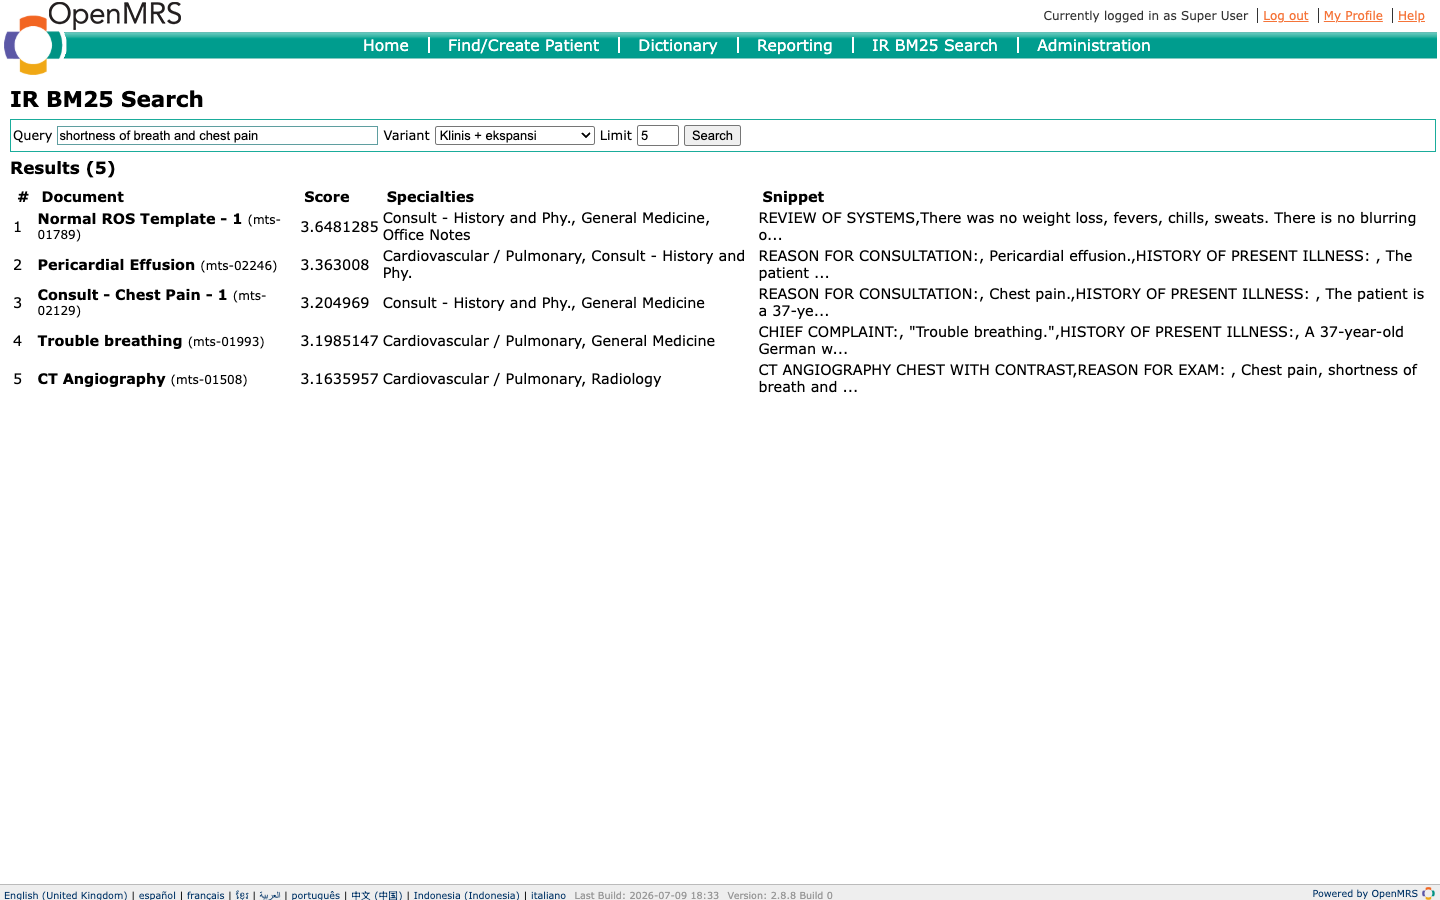
\includegraphics[width=0.85\textwidth]{figures/ui-search}
  \caption{Tampilan pencarian varian tunggal pada modul \texttt{ir-bm25}.}
  \label{fig:ui-search}
\end{figure}

\begin{figure}[h]
  \centering
  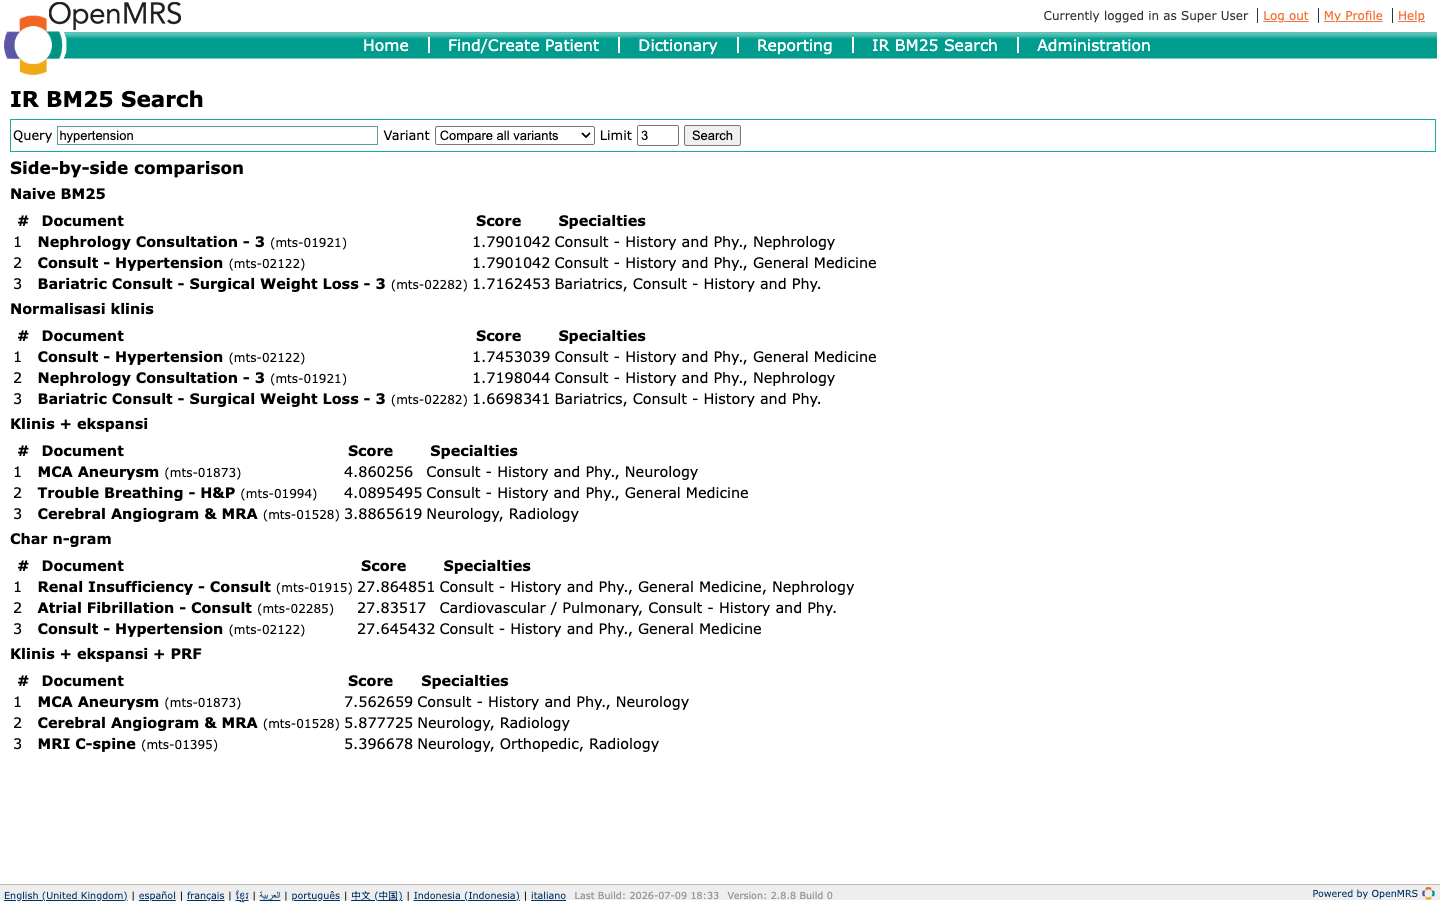
\includegraphics[width=0.85\textwidth]{figures/ui-compare-all}
  \caption{Tampilan mode ``bandingkan semua'' kelima varian pada OpenMRS (query ``hypertension'').}
  \label{fig:ui}
\end{figure}

\section{Hasil dan Evaluasi}
Evaluasi dilakukan pada 50 \textit{query} dengan \textit{cutoff} $K = 10$, menggunakan metrik Precision@10, Recall@10, dan nDCG@10. Hasilnya disajikan pada Tabel~\ref{tab:eval}.

\begin{table}[h]
  \centering
  \caption{Hasil evaluasi ablation study (50 query, K = 10).}
  \label{tab:eval}
  \begin{tabular}{|l|c|c|c|}
    \hline
    \textbf{Varian} & \textbf{P@10} & \textbf{Recall@10} & \textbf{nDCG@10} \\
    \hline
    V0 · Naive BM25 & 0,5400 & \textbf{0,4312} & 0,6832 \\
    \hline
    V1 · Normalisasi klinis & \textbf{0,5420} & 0,4284 & \textbf{0,6865} \\
    \hline
    V2 · Klinis + ekspansi & 0,5120 & 0,4192 & 0,6509 \\
    \hline
    V3 · Char n-gram & 0,5280 & 0,4055 & 0,6446 \\
    \hline
    V4 · Klinis + ekspansi + PRF & 0,5020 & 0,4139 & 0,6186 \\
    \hline
  \end{tabular}
\end{table}

Hasil menunjukkan V1 (normalisasi klinis) berada sedikit di atas baseline naif V0 pada P@10 dan nDCG@10. Besaran selisihnya perlu dibaca dengan hati-hati. Selisih P@10 sebesar 0,0020 pada 50 \textit{query} dengan $K = 10$ setara dengan hanya \emph{satu dokumen} yang berpindah masuk ke sepuluh besar (270 menjadi 271 dokumen relevan dari total 500 posisi terambil), sedangkan selisih nDCG@10 sebesar 0,0033 setara dengan perbaikan relatif 0,48\%. Recall@10 V1 bahkan sedikit lebih rendah daripada V0 (0,4284 berbanding 0,4312), sehingga perbaikannya tidak konsisten di ketiga metrik. Evaluasi ini juga belum menyertakan uji signifikansi statistik, misalnya uji-t berpasangan atau \textit{randomization test} atas skor per-\textit{query}. Karena itu klaim yang dapat dipertanggungjawabkan dari data ini adalah bahwa normalisasi klinis \emph{tidak menurunkan} kualitas peringkat sambil memangkas waktu respons secara substansial (0,68~ms berbanding 2,48~ms per \textit{query}), bukan bahwa ia meningkatkan kualitas peringkat secara meyakinkan.

Nilai Recall@10 pada Tabel~\ref{tab:eval} juga perlu dibaca relatif terhadap plafonnya. Dengan rata-rata 22,3 dokumen relevan per \textit{query} (maksimum 98), \textit{cutoff} $K = 10$ membuat recall maksimum yang secara teoretis dapat dicapai hanya 0,6762, bukan 1,0. Dengan demikian angka 0,4312 pada V0 setara dengan sekitar 64\% dari plafon yang mungkin dicapai pada protokol ini.

Secara fungsional, ekspansi singkatan terverifikasi bekerja: \textit{query} ``CKD'' berhasil menemukan dokumen berjudul ``Chronic Kidney Disease - Followup'', dan \textit{query} ``hypertension'' menemukan dokumen yang memuat singkatan ``HTN''.

\subsection{Keterbatasan Evaluasi}
\label{sub:keterbatasan}
Penurunan presisi pada V2, V3, dan V4 sebaiknya tidak langsung dibaca sebagai bukti bahwa ekspansi merugikan. Terdapat keterbatasan struktural pada qrels yang digunakan: penilaian relevansi dibangun dari kolom metadata (\texttt{keywords}, \texttt{sample\_name}, \texttt{description}), sedangkan yang diindeks dan diperingkat oleh mesin IR adalah kolom \texttt{transcription}. Pengukuran langsung pada dataset menunjukkan ketimpangan yang besar antara keduanya, sebagaimana dirangkum pada Tabel~\ref{tab:keterbatasan}.

\begin{table}[h]
  \centering
  \caption{Ketimpangan antara ranah penilaian relevansi dan ranah pengindeksan.}
  \label{tab:keterbatasan}
  \begin{tabular}{|>{\raggedright\arraybackslash}p{10.2cm}|r|}
    \hline
    \textbf{Aspek} & \textbf{Nilai} \\
    \hline
    Panjang rata-rata field penilaian (\texttt{keywords} + \texttt{sample\_name} + \texttt{description}) & 44 token \\
    \hline
    Panjang rata-rata field yang diindeks (\texttt{transcription}) & 466 token \\
    \hline
    Rasio ketimpangan & 10,6$\times$ \\
    \hline
    Dokumen tanpa \texttt{keywords} sama sekali & 526 (22,7\%) \\
    \hline
    Dokumen yang pernah dinilai relevan untuk suatu \textit{query} & 841 (36,3\%) \\
    \hline
  \end{tabular}
\end{table}

Akibatnya, dokumen yang \texttt{transcription}-nya benar-benar membahas suatu kondisi klinis tetapi metadatanya tidak memuat istilah tersebut akan dinilai tidak relevan, meskipun dokumen itu sesungguhnya relevan dan berhasil ditemukan sistem. Bias ini bekerja paling keras justru terhadap varian yang dirancang menembus permukaan teks, yaitu V2 (ekspansi sinonim), V3 (\textit{char n-gram}), dan V4 (PRF), karena dokumen tambahan yang mereka temukan cenderung merupakan kecocokan pada tubuh narasi, bukan pada metadata. Dengan kata lain, sebagian dari apa yang terukur sebagai penurunan presisi pada Tabel~\ref{tab:eval} berpotensi merupakan artefak protokol penilaian, bukan kegagalan varian tersebut.

Karena itu, angka pada Tabel~\ref{tab:eval} lebih tepat dibaca sebagai perbandingan antarvarian pada satu protokol penilaian yang sama, bukan sebagai estimasi kualitas absolut sistem. Menghilangkan keterbatasan ini memerlukan \textit{relevance judgment} yang dinilai langsung pada isi \texttt{transcription}, idealnya oleh penilai dengan latar klinis.

\section{Kesimpulan}
Proyek ini berhasil mengimplementasikan mesin \textit{ranked retrieval} BM25 dengan lapisan normalisasi dan ekspansi klinis, mengintegrasikannya ke OpenMRS sebagai modul tambahan, serta mengevaluasinya melalui ablation study lima varian pada dataset MTSamples. Validasi berbasis dataset menunjukkan bahwa penanda negasi, istilah majemuk, dan singkatan medis muncul pada sebagian besar dokumen, sehingga tokenisasi klinis bukan sekadar asumsi. Hasil evaluasi menunjukkan normalisasi klinis (V1) berada tipis di atas baseline naif, namun selisihnya berada dalam rentang \textit{noise} dan belum diuji signifikansinya, sehingga simpulan yang dapat ditegakkan adalah bahwa lapisan tokenisasi klinis tidak menurunkan kualitas peringkat sambil mempercepat waktu respons. Analisis keterbatasan pada Subbab~\ref{sub:keterbatasan} menunjukkan bahwa penurunan presisi pada varian ekspansi sebagian besar dapat dijelaskan oleh protokol qrels yang menilai relevansi dari metadata, sementara sistem memeringkat berdasarkan isi transkripsi. Modul teruji berjalan pada OpenMRS 2.8.8 dan siap digunakan sebagai purwarupa pencarian cerdas bagi tenaga medis.

\section{Saran}
Berdasarkan keterbatasan yang teridentifikasi, pengembangan lanjutan diarahkan pada empat hal berikut.
\begin{enumerate}
    \item Menyusun \textit{relevance judgment} yang dinilai langsung pada isi \texttt{transcription}, bukan pada kolom metadata, idealnya melalui penilaian manual oleh tenaga dengan latar klinis, sehingga varian ekspansi dinilai pada ranah yang sama dengan ranah pengindeksan.
    \item Menambahkan keluaran skor per-\textit{query} pada \texttt{EvalRunner} agar uji signifikansi statistik (uji-t berpasangan atau \textit{randomization test}) dapat dijalankan, sehingga perbandingan antarvarian memiliki dasar inferensial.
    \item Memperluas cakupan \textit{lexicon} klinis dari kamus kurasi manual (13 penanda negasi, 28 istilah majemuk, 28 singkatan, 15 grup sinonim) menuju sumber terstandar seperti UMLS atau SNOMED~CT, agar cakupan singkatan yang kini baru 28,8\% dapat ditingkatkan.
    \item Melakukan \textit{tuning} parameter $k_1$ dan $b$ per varian, serta mengevaluasi pada \textit{cutoff} $K$ yang lebih besar agar Recall@K tidak terkendala plafon rendah akibat banyaknya dokumen relevan per \textit{query}.
\end{enumerate}

\clearpage
\bibliographystyle{agm-dkk}
\bibliography{references}

\end{document}
